\chapter{SmartDebug工具设计与实现}
\label{cha:impl}

\section{引言}
“生成-检验”系统的目的是自动修复程序中的代码错误,使其能够通过对应的测试集。在当前的研究状态下,“生成-检验”系统修复正确率和效率都与实际应用有一定距离。在前几个章节中,本文提出了针对搜索引擎模块的“预过滤”优化算法、“交互式调试”框架扩展以及“针对特定类型错误的扩展框架”几种技术方案,目的都是提高“生成-检验”系统的修复准确率和系统效率。在本章中,我们将所提出的技术实现为工具原型SmartDebug,从使用者角度介绍系统功能,并以一个示例程序说明系统的使用方式。

\section{功能模块}
SmartDebug工具的核心功能是为开发人员提供程序的修复建议,提高程序修复速度。为方便开发人员使用,SmartDebug实现在Eclipse插件平台上,与Eclipse IDE无缝集成在一起。

图\ref{fig:example-1}展示了SmartDebug的工具界面。其中,代码编辑器、调试窗口、JUnit测试界面等都是Eclipse Java调试视图中的一部分,SmartDebug加入的窗口是“检查点(Checkpoints)”管理窗口和“修复建议列表(Fix Suggestions)”窗口。其中,检查点窗口管理和展示所有已注册的检查点,检查点的状态表示着当前调试任务的进展情况,因此我们也将其称为调试进度管理窗口。这两个窗口分别对应系统的两个主要功能模块,即检查点管理模块和修复建议提示与应用模块。

\subsection{检查点管理模块}
检查点管理模块为用户提供查看和修改代码中注册的检查点的接口。如图所示,检查点按照其与测试用例的所属关系以树形结构展示在面板中,检查点的两个属性则以列表方式显示。每个检查点的状态以不同颜色图标显示,绿色表示已通过,黑色表示不通过,黄色表示未知。使用者可以在面板中完成对检查点的增、删、改、查操作。其中,增加和修改检查点功能只在程序执行某一测试用例过程中触发,这是由于检查点的增加和修改意味着开发人员在观察程序运行状态时得到了某一判断。删除则可以通过选中某一检查点,点击右上角的“X”型按钮在任意时刻完成。

\subsection{修复建议提示与应用模块}

修复建议列表窗口展示了在当前调试目标下系统找到的符合要求的修复建议。在使用过程中,系统可能会产生多条修复建议,这说明程序使用其中任一一条修复建议都可以完成此次修复会话的调试目标,此时开发人员需要逐一检查这些建议条目,并选择合适的修复建议,点击右上角“A”字按钮,则程序将被修改。

\section{应用示例}
本节以一个具体调试任务为例说明SmartDebug的使用方法。代码\ref{code:fix-example}来自于本校研究生Java程序水平考试中某位同学答题时程序的一个中间版本。题目的要求是,给定一个素数,找出将其分解为不大于它本身的连续素数之和(包括素数本身)的方法数目。题目给出了两个测试数据点,2和53,对应的输出分别是1和2。

代码\ref{code:fix-example}包含主程序代码和测试程序代码。在主程序中,算法分为两个步骤,第一是计算出不大于输入\texttt{input}的素数列表,第二是在素数列表中计算连续素数的和,查找有多少次与\texttt{input}相等。代码中共有两处错误,第一是在\texttt{isPrime}方法中判断一个数是否是素数时第26行的判断条件写错,应将\texttt{i<=n}改为\texttt{i<n}。第二是在\texttt{split}方法中求连续素数和时第41行上的列表下标写错,应将\texttt{j}写成\texttt{i}。测试代码分别对应题目给出的两个数据点。

\begin{lstlisting}[caption=应用示例,frame=single,language=Java,numbers=left,basicstyle=\ttfamily\footnotesize,label={code:fix-example},tabsize=2]
//----------------主程序-------------------------------------
public class Main {
	
	public static int splitCount(int input){
		ArrayList<Integer> primeList = getPrimeList(input);
		int count = split(input, primeList);
		return count;
	}
	
	private static ArrayList<Integer> getPrimeList(int n){		
		ArrayList<Integer> list = new ArrayList<Integer>();
		for(int i=1;i<=n;i++){
			if(isPrime(i)){
				list.add(i);
			}
		}
		return list;
	}
	
	private static boolean isPrime(int n){
		if(n == 1)
			return false;
		if(n==2)
			return true;
		int i = 2;
			while (i<=n) { // ERROR HERE: it should be (i < n)
				if((n % i)==0){
				return false;
			}
			i++;
		}
		return true;
	}

	private static int split(int n, ArrayList<Integer> list){
		int count=0;
		int size = list.size();
		for(int i=0;i<size;i++){
			int sum = 0;			
			for(int j=i;j<size;j++){
				sum+=list.get(i); // ERROR HERE: it should be get(j)
				if(sum==n){
					count++;
				}
			}
		}
		return count;
	}
}

//----------------------测试代码---------------------------------
public class MainTest {

	@Test
	public void test1(){
		int input = 2;
		int result = Main.splitCount(input);
		Assert.assertEquals(1, result);
	}

	@Test
	public void test2(){
		int input = 53;
		int result = Main.splitCount(input);
		Assert.assertEquals(2, result);
	}
}
\end{lstlisting}

使用SmartDebug完成调试任务的流程如下。首先,执行JUnit测试,会发现测试用例\texttt{test2}不通过,于是在主程序入口处加断点,单步调试该测试用例。当程序执行到图\ref{fig:example-1}中所示位置时,程序中变量\texttt{primeList}内容不对,应包含53以下的所有素数。因此,我们在此处按住Ctrl并左键单击代码编辑框左边栏,加入第一个检查点。

\begin{figure}
	\centering
	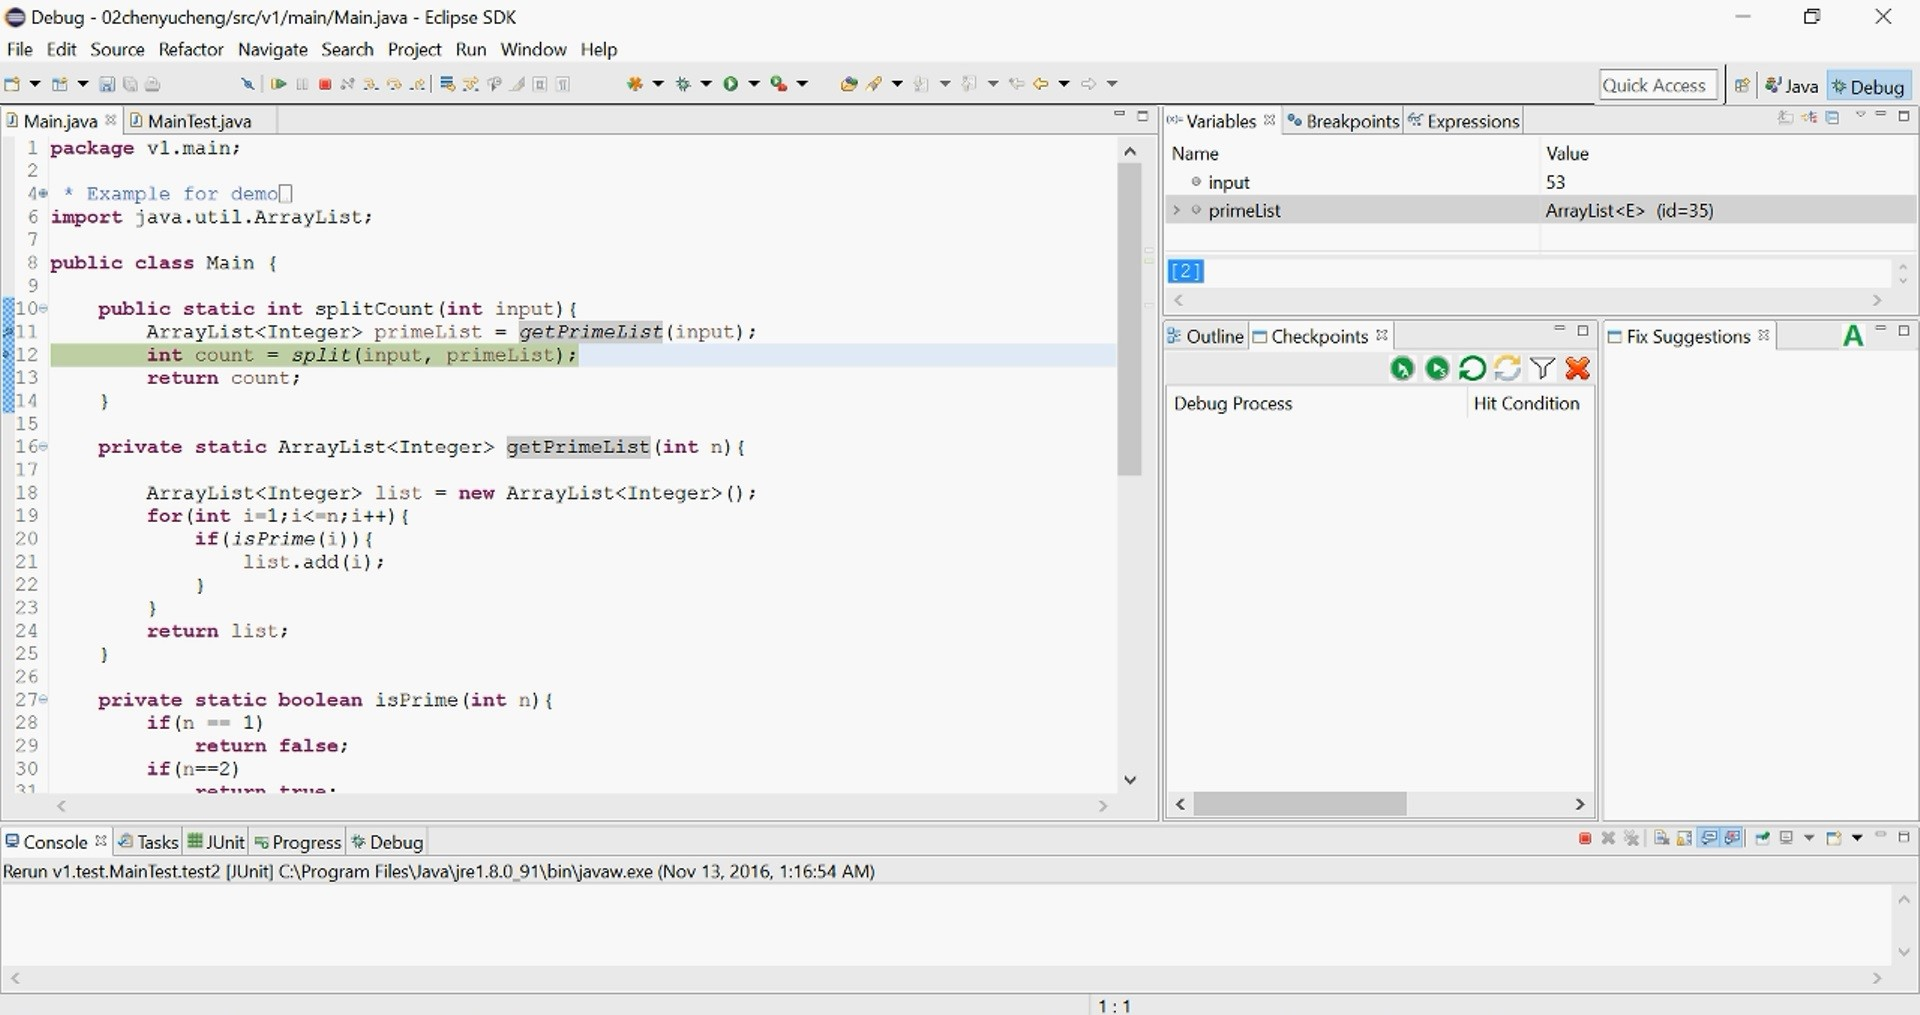
\includegraphics[width=1\linewidth]{chap05/1}
	\caption{(1)}
	\label{fig:example-1}
\end{figure}

图\ref{fig:example-2}展示了检查点属性输入对话框。对话框左边栏输入此时执行到当前位置的次数,右边栏键入此程序状态应满足的条件。这里由于这一位置只执行一次,则右边的条件在每次程序执行到此处时都需成立,因此我们在左侧直接输入“true”表示右侧条件恒成立。在右侧我们输入条件表示此处\texttt{primeList}的大小应至少为2。点击确定,则此时可看到检查点管理面板中已注册了这一检查点(图\ref{fig:example-3}),而代码编辑框左边栏对应位置也有了标志。

\begin{figure}
	\centering
	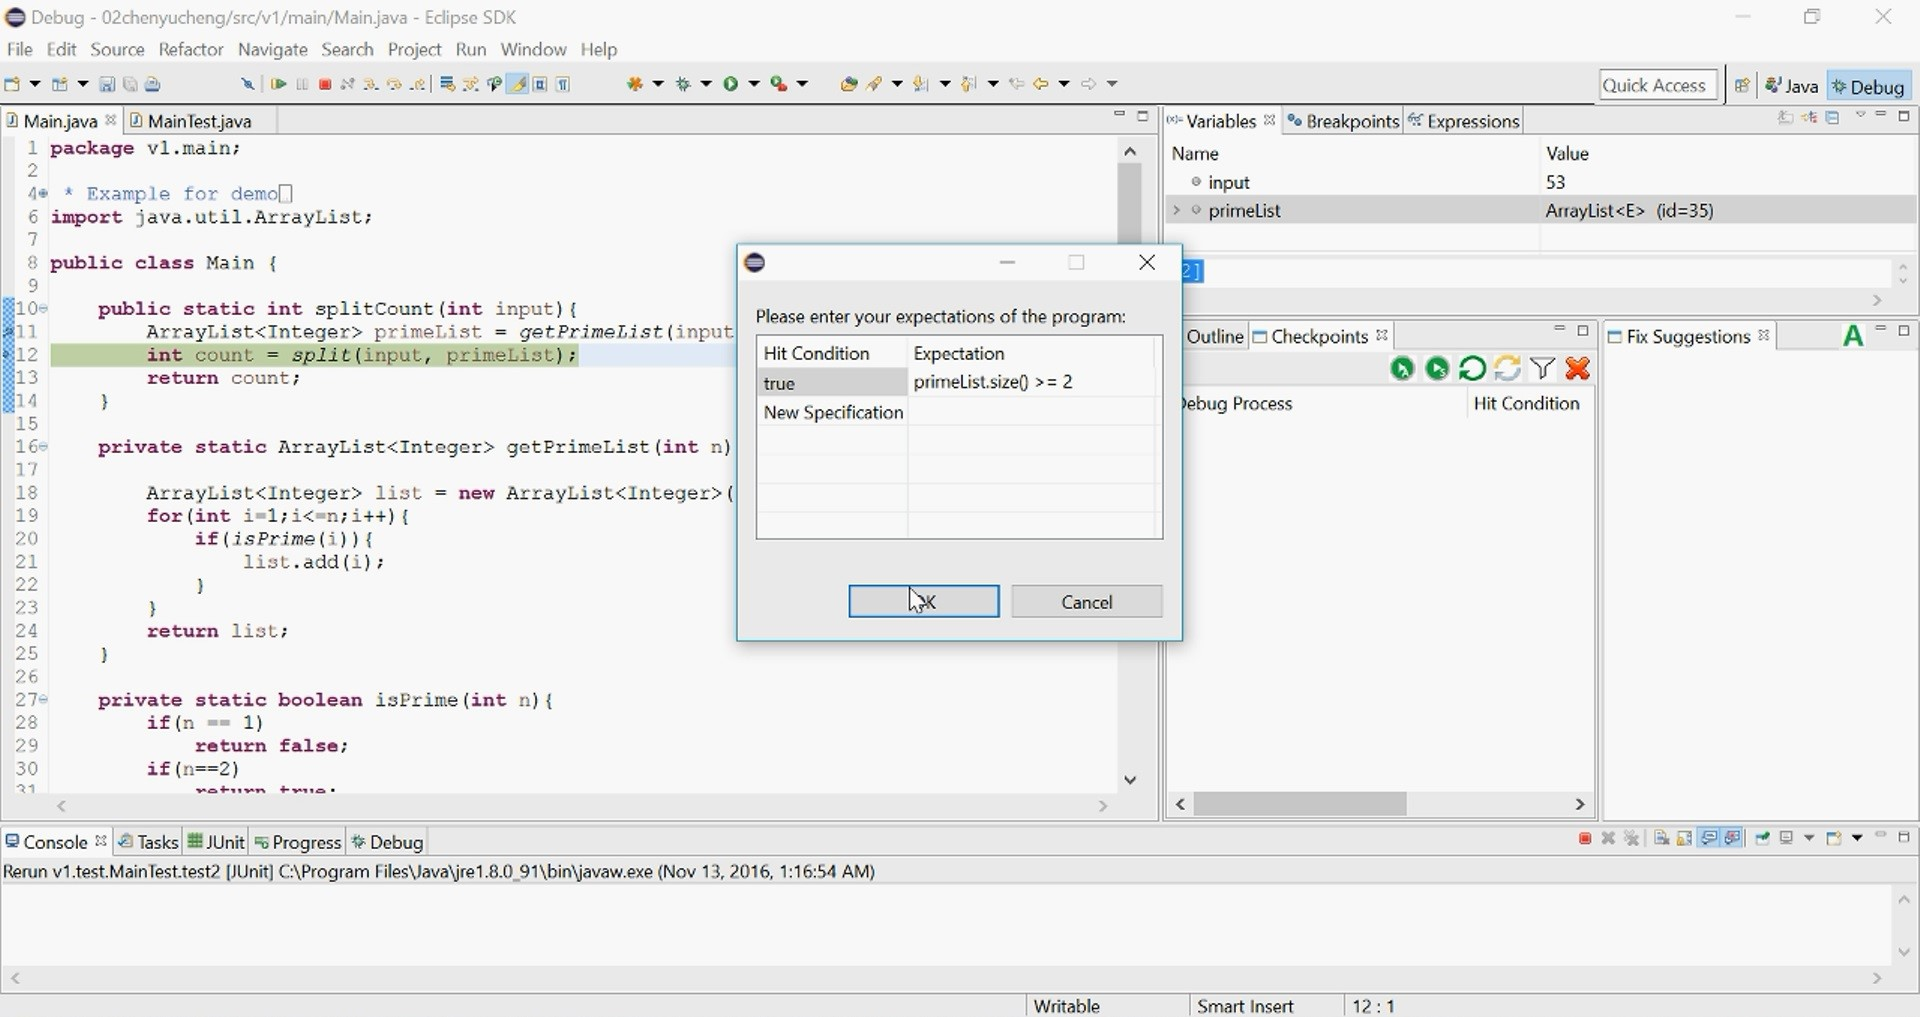
\includegraphics[width=1\linewidth]{chap05/2}
	\caption{(2)}
	\label{fig:example-2}
\end{figure}
\begin{figure}
	\centering
	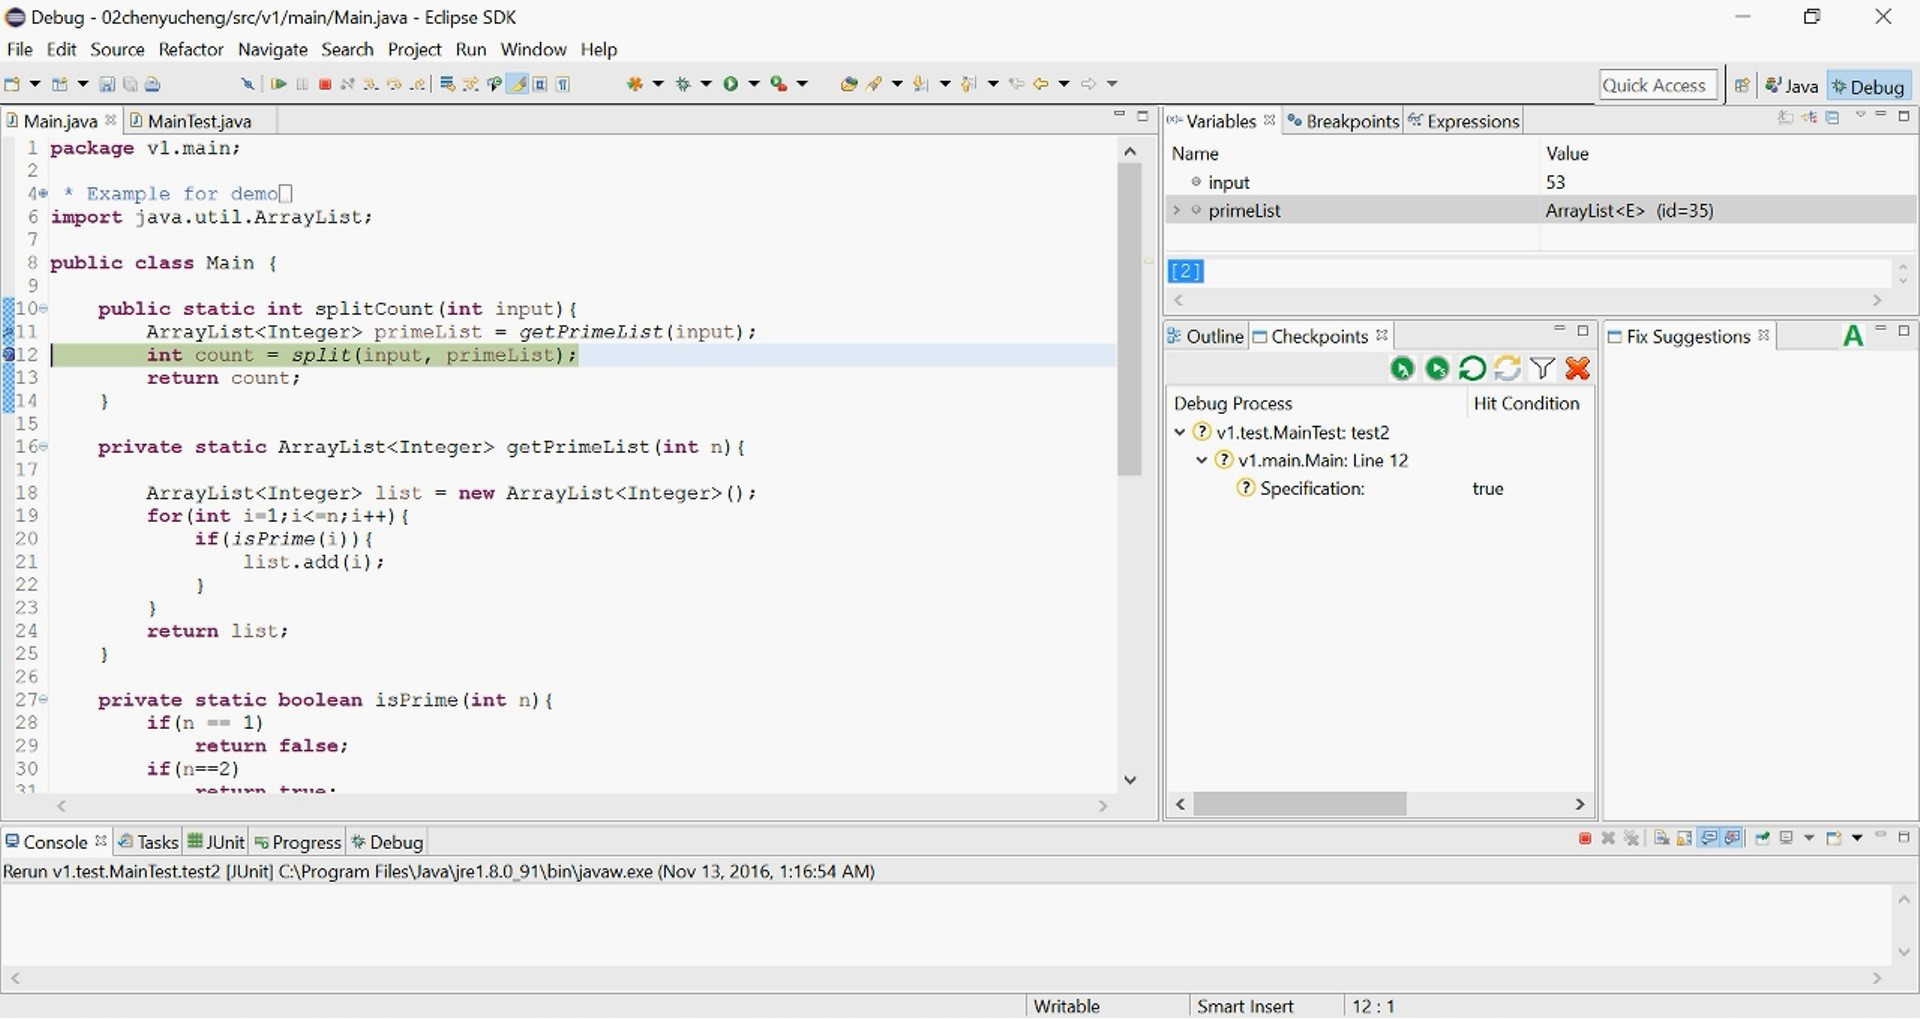
\includegraphics[width=1\linewidth]{chap05/3}
	\caption{(3)}
	\label{fig:example-3}
\end{figure}

程序继续执行,在图\ref{fig:example-4}位置上,变量\texttt{count}表示程序找到的素数分拆方法数,此时该变量的值应为2,因此在此处可以类似的加入检查点,将条件设置为“\texttt{count==2}”。点击确定,则如图\ref{fig:example-5}所示,新的检查点被添加。此时,点击“刷新”按钮,系统将执行程序,并计算检查点当前的状态。如图中所示,首先被加入的检查点状态是“不通过”,而后加入的检查点状态是“未知”,这是由于调试进度控制模块在更新检查点状态时,一旦在一个测试用例执行过程中遇到一个不通过的检查点就会停止运行,这使得调试任务按照一定顺序逐步完成。
\begin{figure}
	\centering
	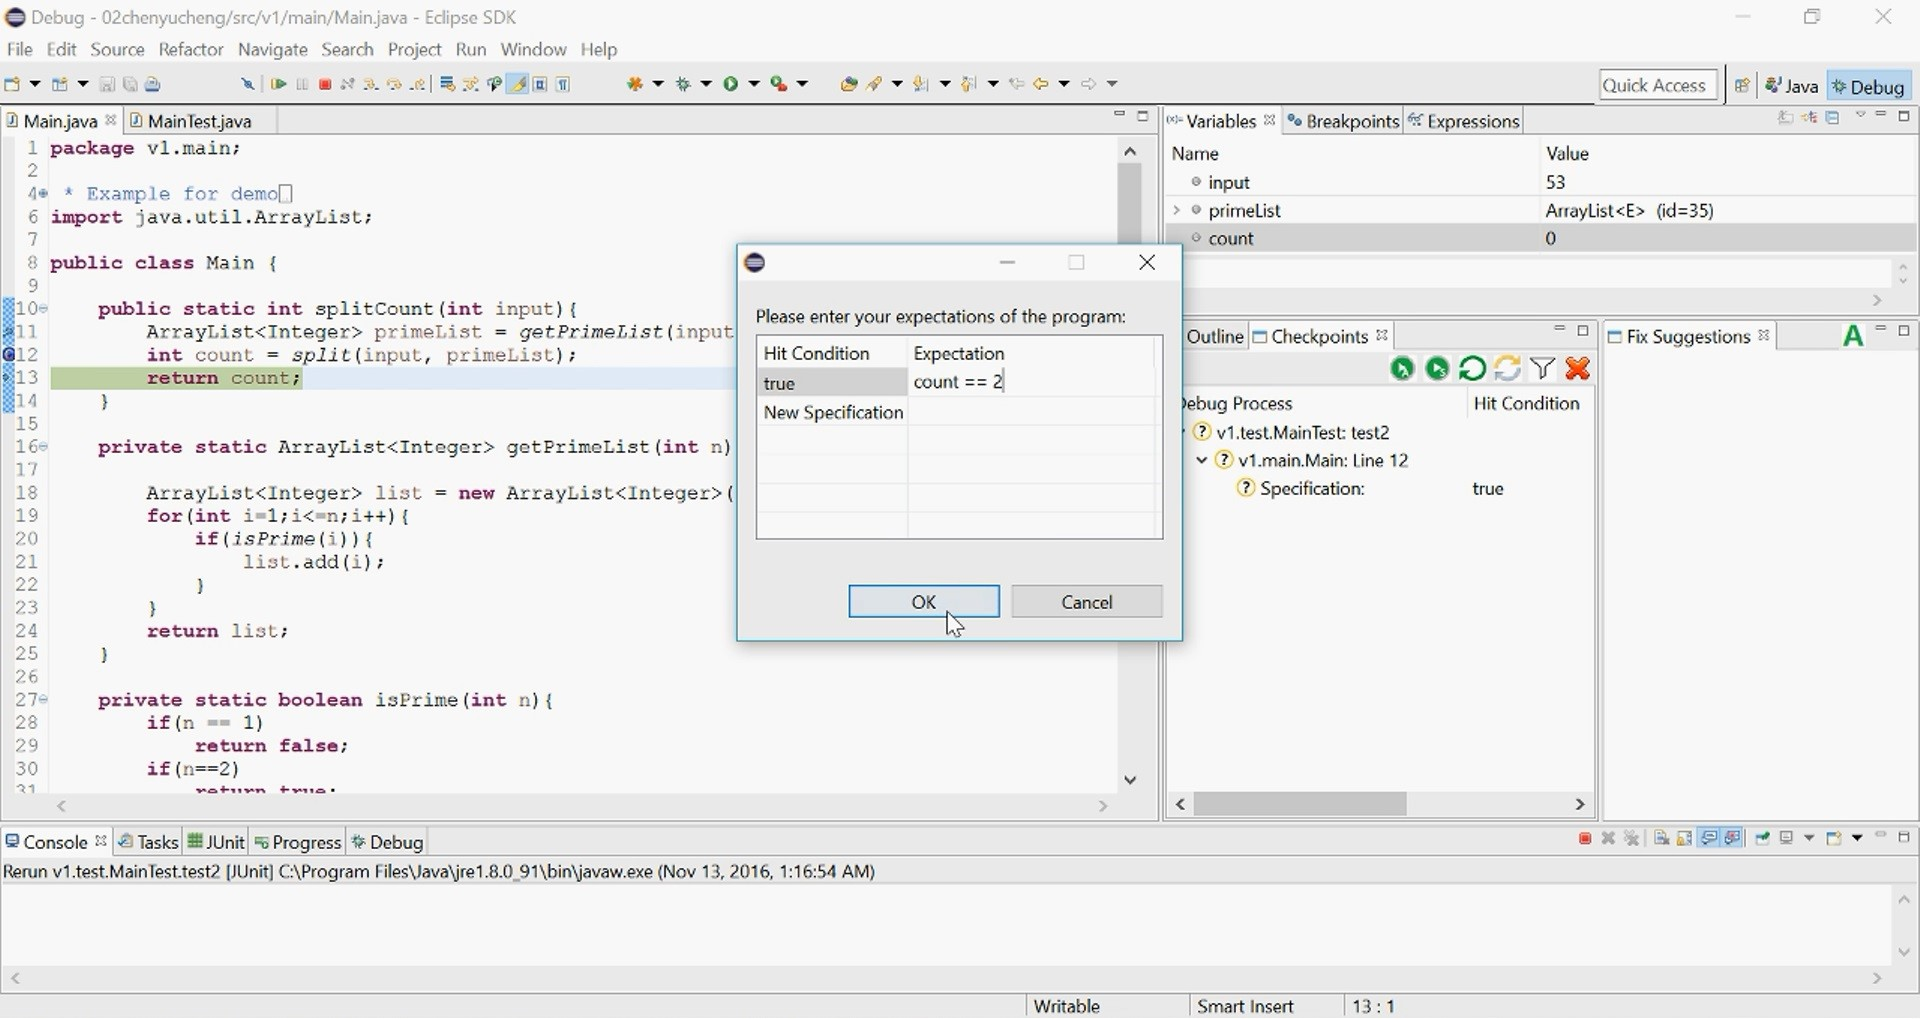
\includegraphics[width=1\linewidth]{chap05/4}
	\caption{(4)}
	\label{fig:example-4}
\end{figure}
\begin{figure}
	\centering
	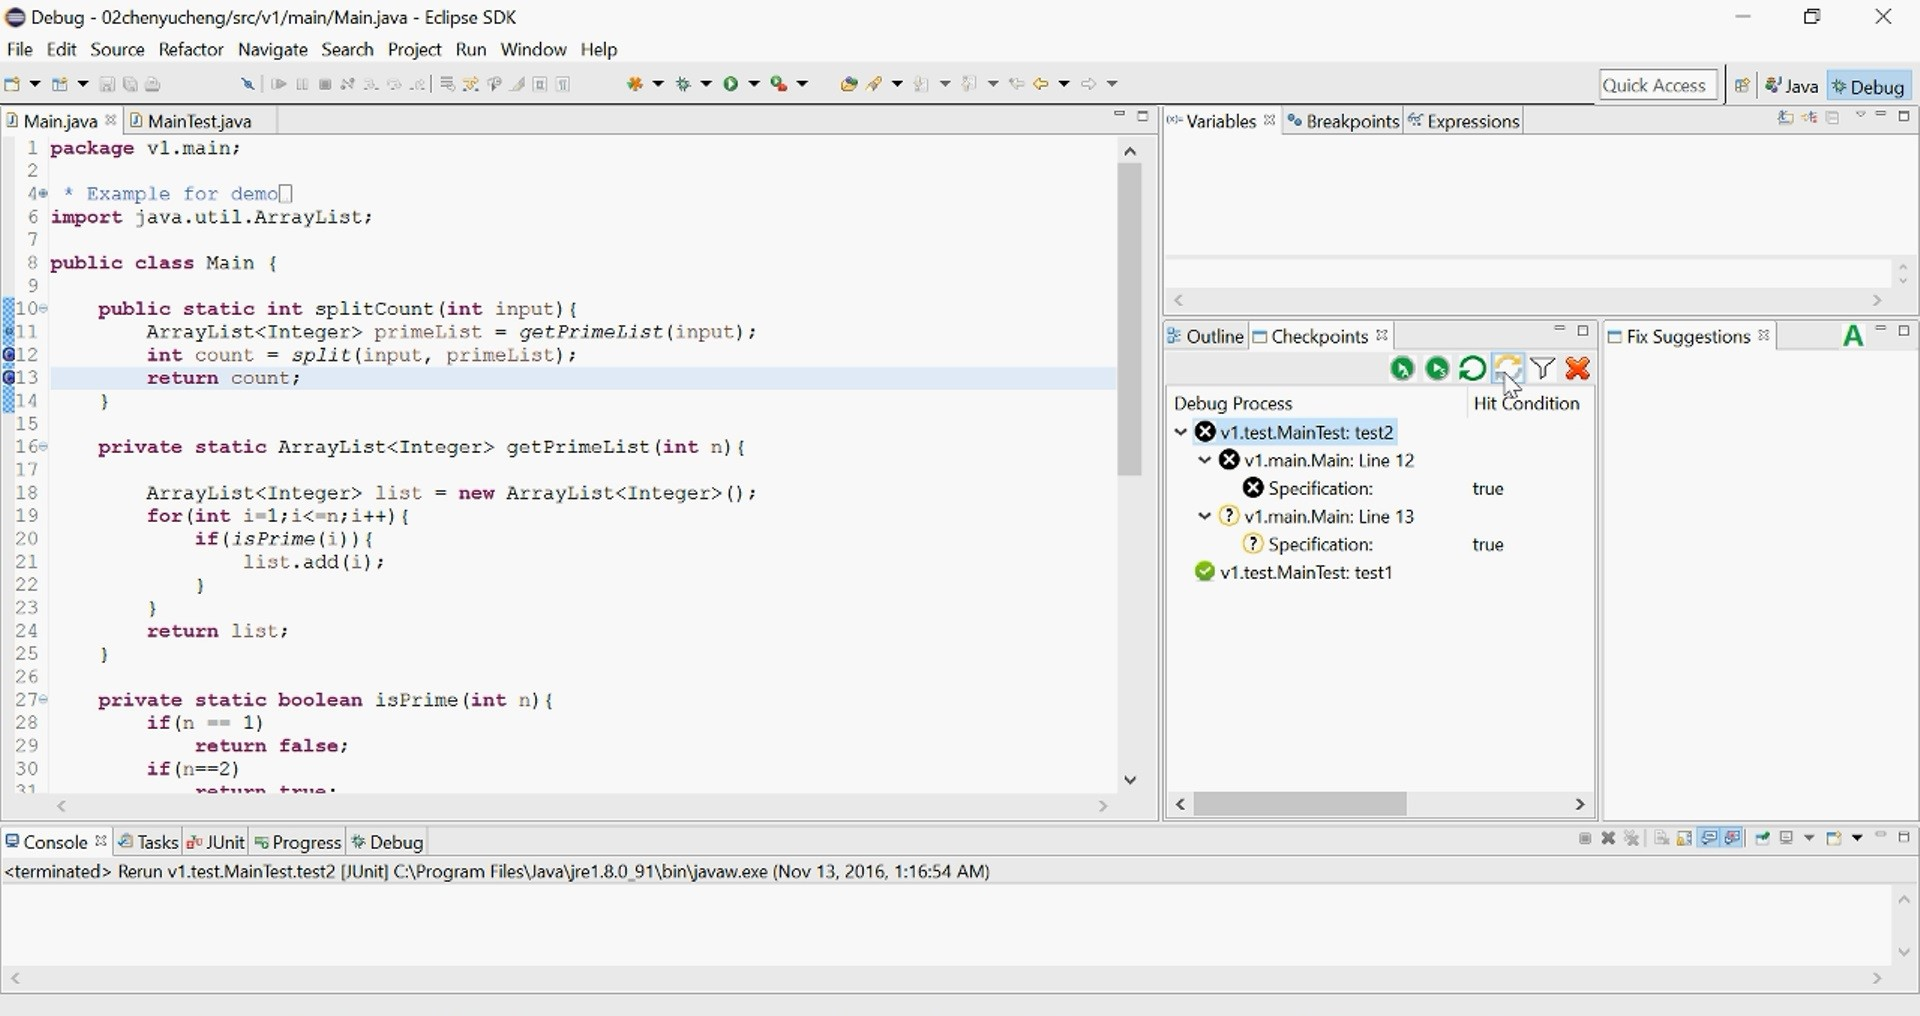
\includegraphics[width=1\linewidth]{chap05/5}
	\caption{(5)}
	\label{fig:example-5}
\end{figure}

图\ref{fig:example-6}标出了“预过滤”优化算法的启用按钮。由于“预过滤”算法有时会将有效的修复建议滤除,产生一定的漏报,因此SmartDebug提供开关供用户选择是否启用这一功能。
\begin{figure}
	\centering
	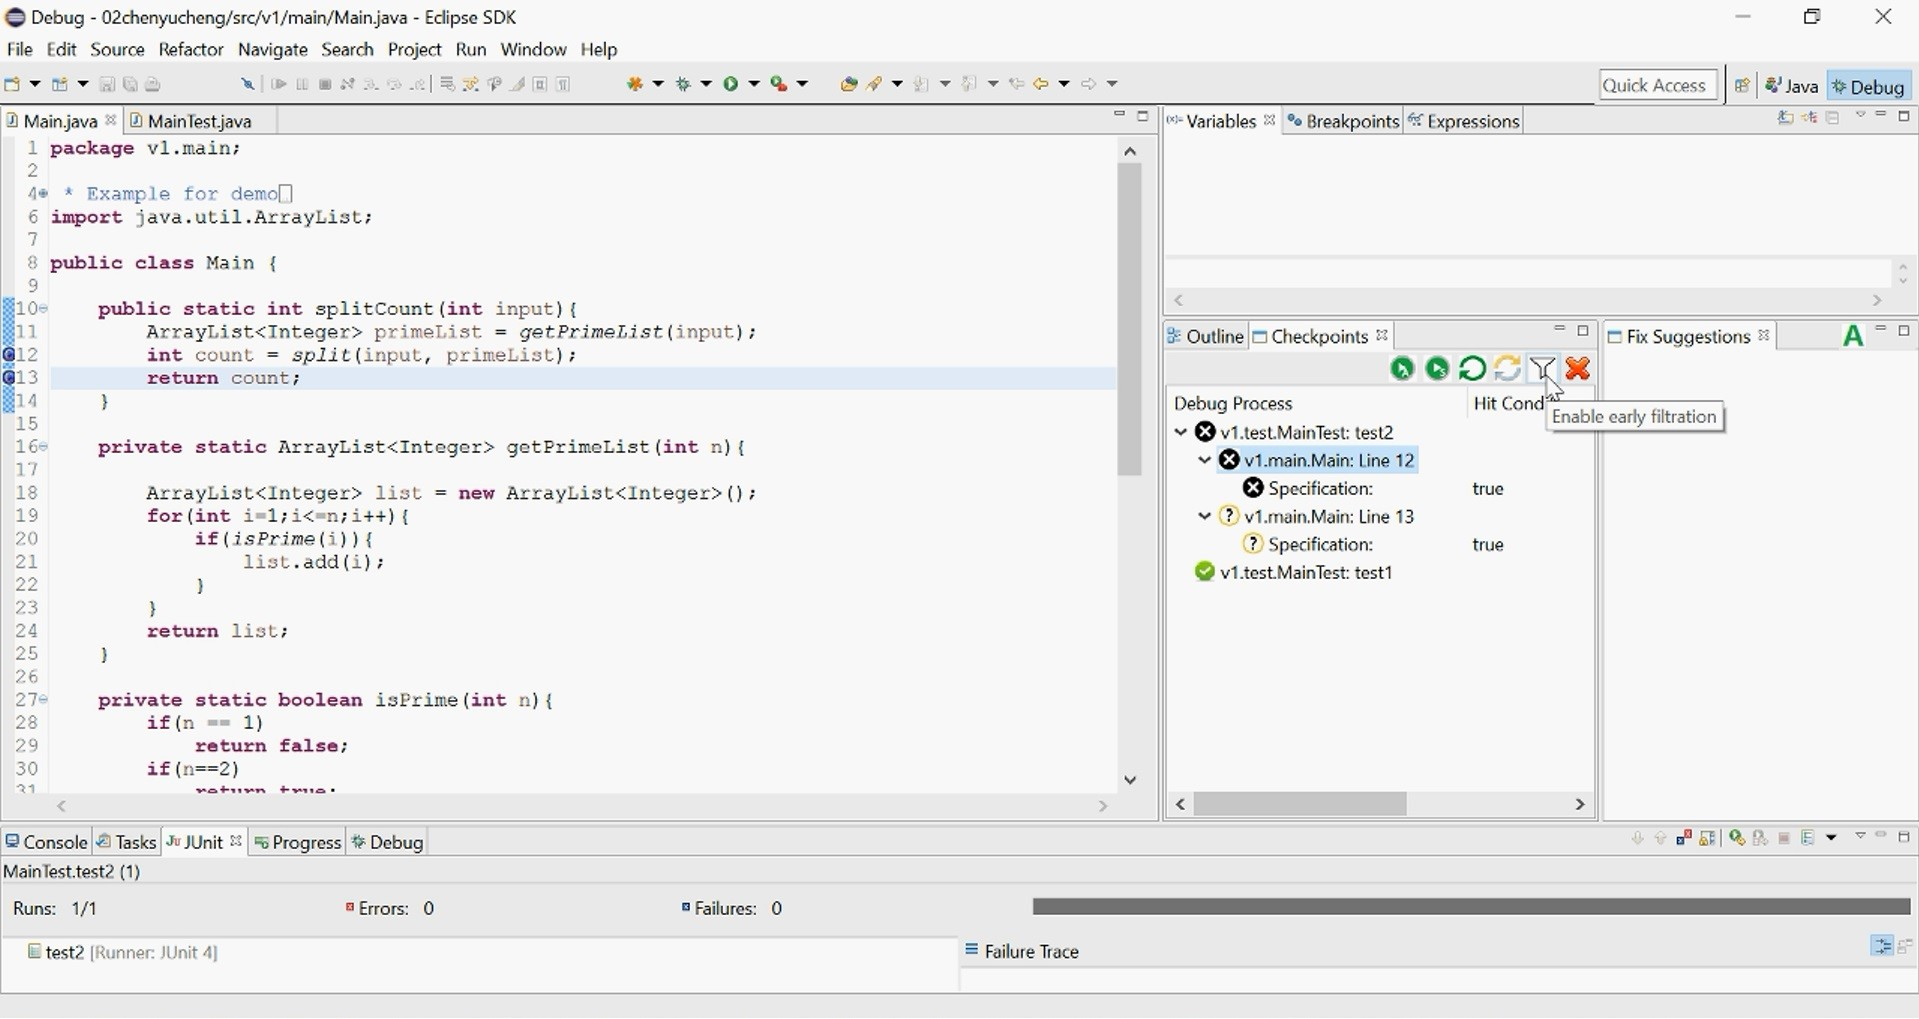
\includegraphics[width=1\linewidth]{chap05/6}
	\caption{(6)}
	\label{fig:example-6}
\end{figure}
在设置检查点后,使用者可以选择当前一个状态为“不通过”的检查点作为调试目标,点击“开始调试”按钮,则系统进入修复建议搜索状态。图\ref{fig:example-8}展示了搜索过程中系统的运行状态。SmartDebug使用了Eclipse提供的进度提示框方便使用者控制搜索过程。使用者可随时点击“取消”暂停当前搜索过程,也可在暂停后点击“继续”按钮继续刚才的搜索过程。搜索过程中合理的修复建议会实时被添加到修复建议列表框中。
\begin{figure}
	\centering
	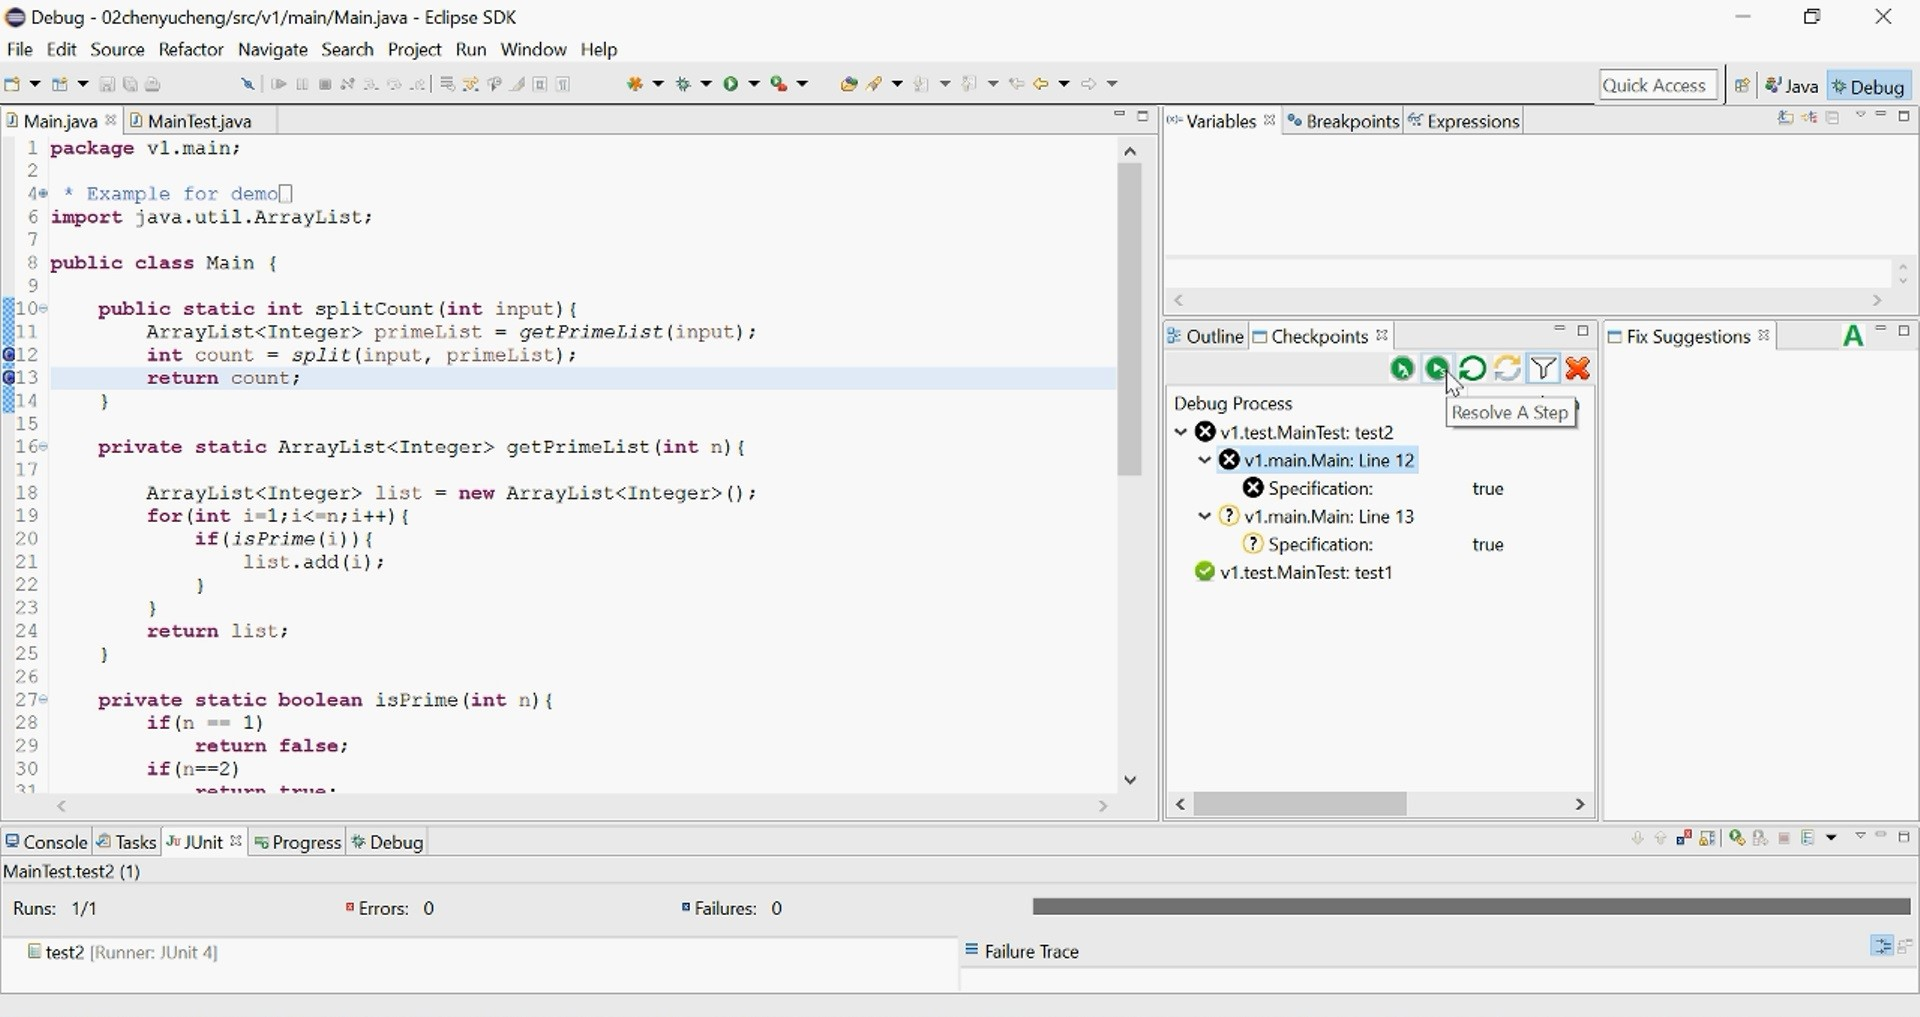
\includegraphics[width=1\linewidth]{chap05/7}
	\caption{(7)}
	\label{fig:example-7}
\end{figure}

\begin{figure}
	\centering
	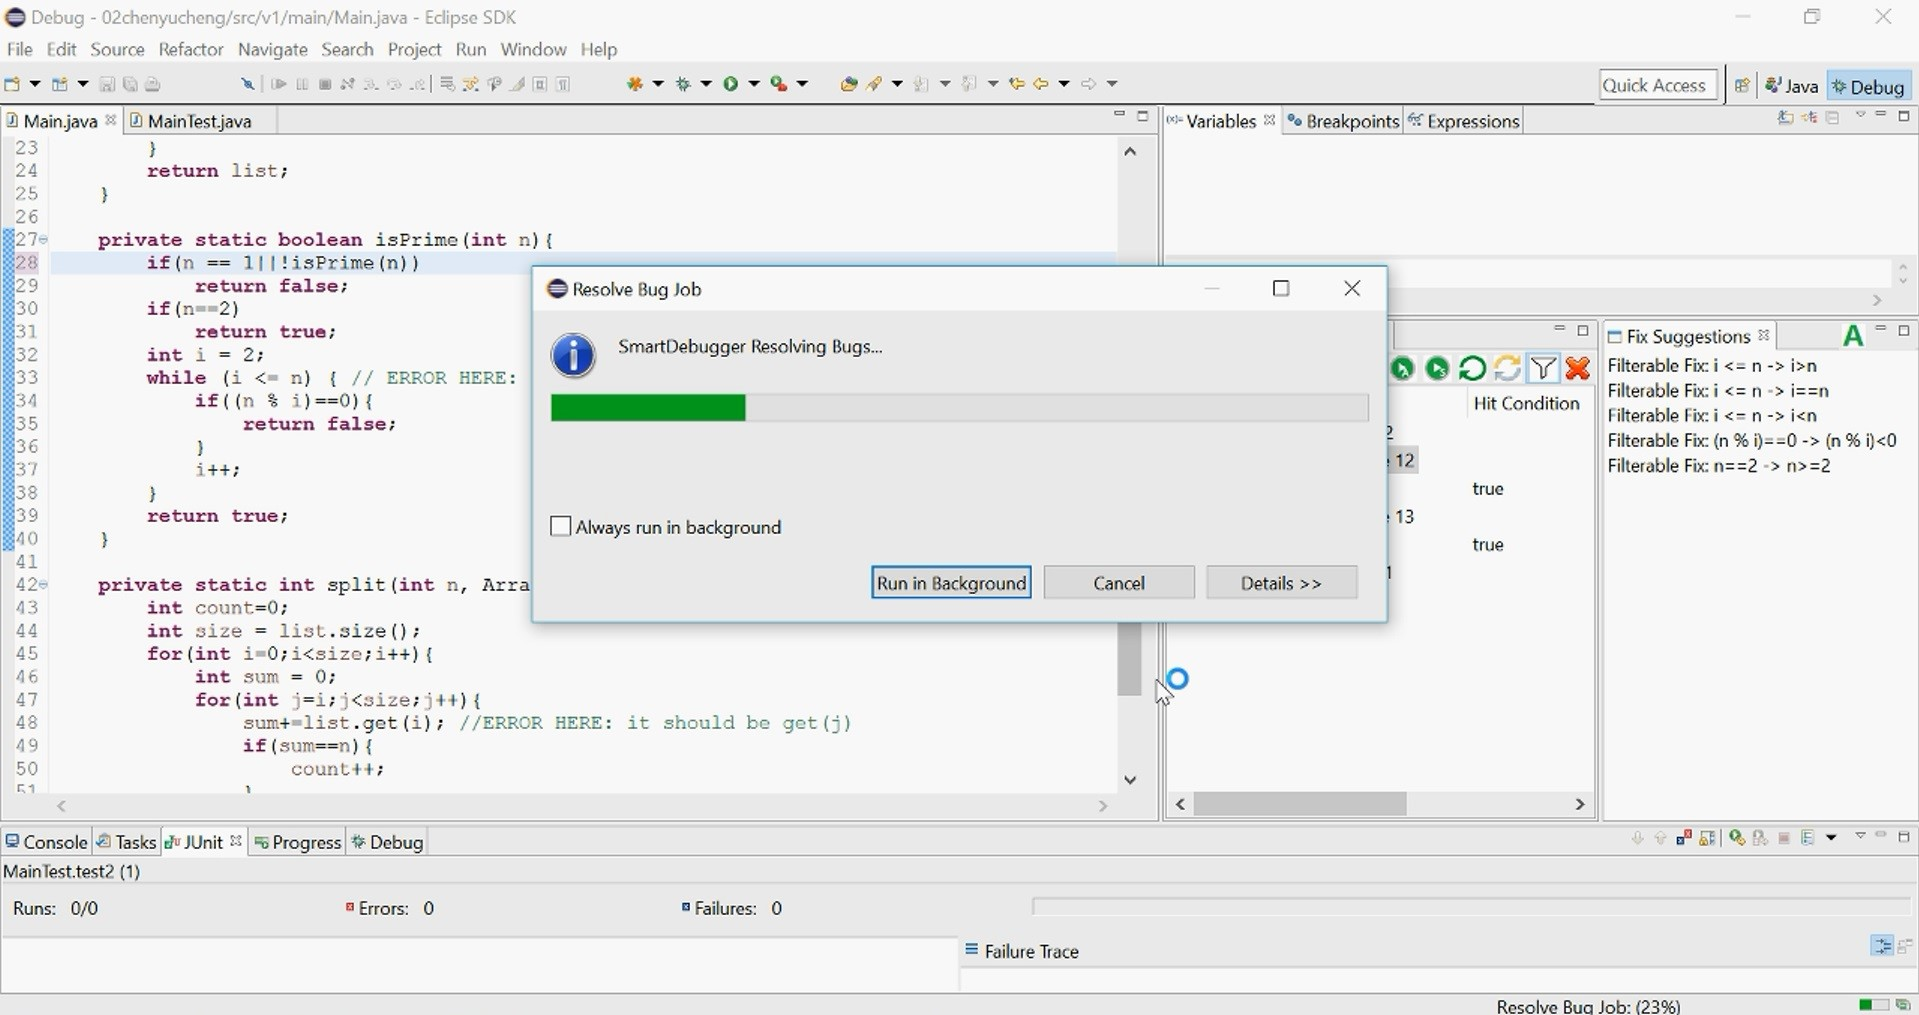
\includegraphics[width=1\linewidth]{chap05/8}
	\caption{(8)}
	\label{fig:example-8}
\end{figure}
当搜索过程结束时,使用者可在右侧修复建议列表框中选择合适的修改建议,点击“A”字按钮,则程序会被相应修改。

完成修改后,刷新检查点管理面板,可以看到第一个检查点状态已变成“通过”,而第二个检查点状态变为“不通过”。此时,可重复上述步骤,启动新的修复会话,生成新的修复建议(图\ref{fig:example-11}),将其应用于程序。此时再刷新检查点管理面板,可以看到所有检查点都通过(图\ref{fig:example-12}),重新执行测试用例,也可看到程序通过了测试。至此,调试任务已经完成。

\begin{figure}
	\centering
	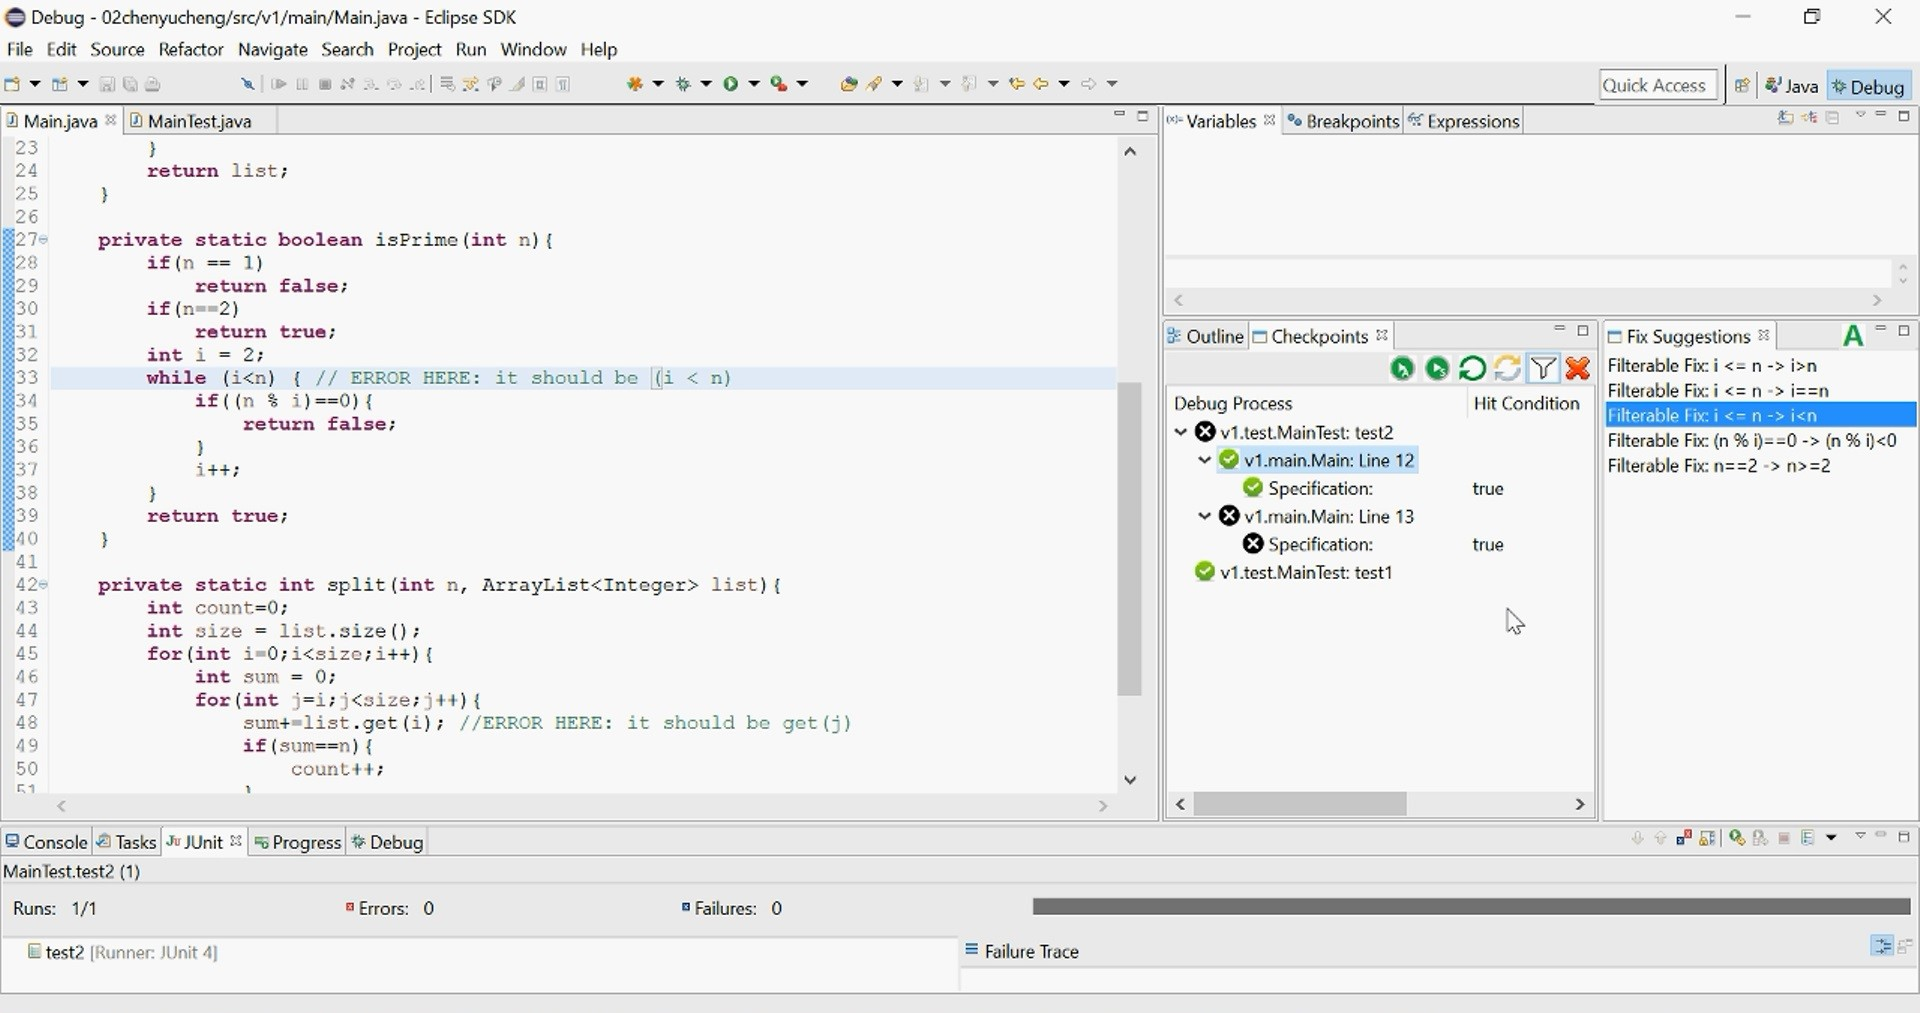
\includegraphics[width=1\linewidth]{chap05/10}
	\caption{(9)}
	\label{fig:example-10}
\end{figure}
\begin{figure}
	\centering
	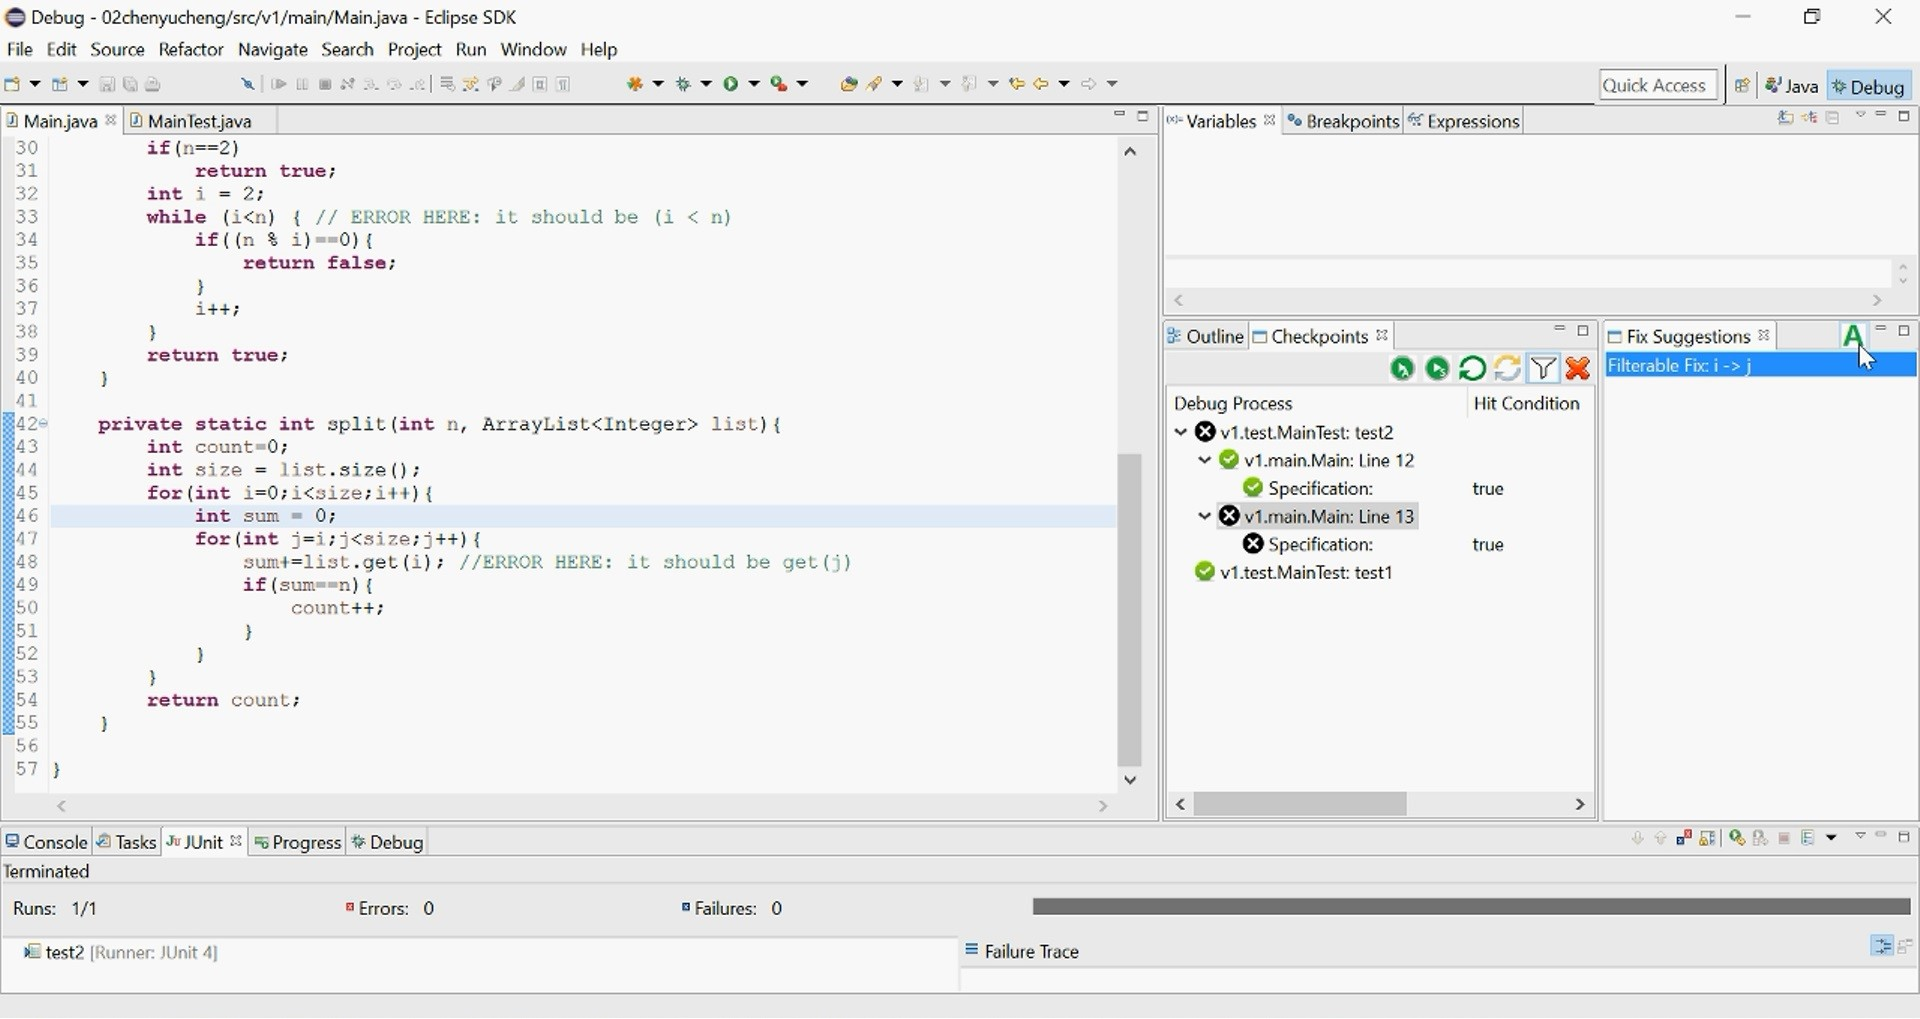
\includegraphics[width=1\linewidth]{chap05/11}
	\caption{(10)}
	\label{fig:example-11}
\end{figure}
\begin{figure}
	\centering
	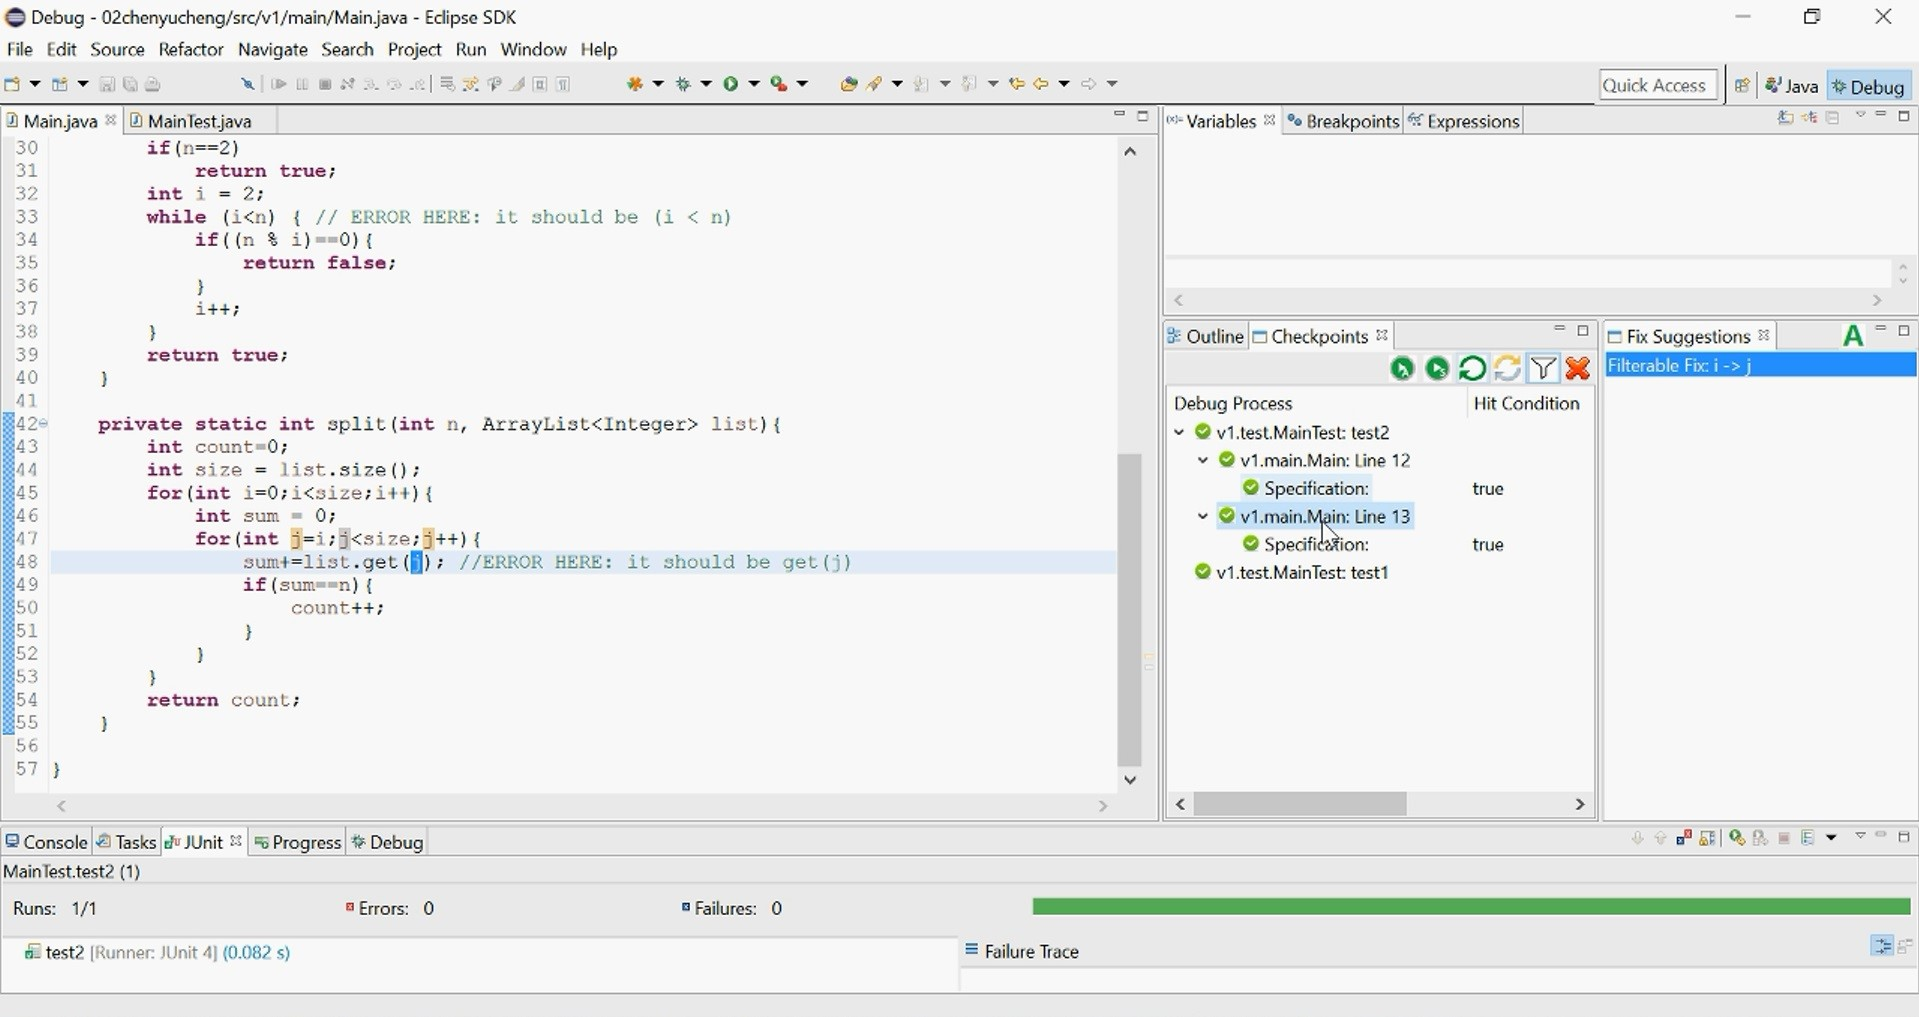
\includegraphics[width=1\linewidth]{chap05/12}
	\caption{(11)}
	\label{fig:example-12}
\end{figure}

\section{本章小结}

基于前两章的研究成果,本文实现了系统SmartDeubg工具原型。本章介绍了SmartDebug工具的主要功能,并以一个实际调试任务展示了工具的使用方式。